\chapter{روش پیشنهادی}
%\thispagestyle{empty}

\section{مقدمه}
در بخش قبلی با برخی پیشنیاز‌های مربوط به مسئله اصلی و برخی از مطالعات انجام شده در استفاده از دفتر سفارشات آشنا شدیم. در این بخش قصد داریم تا روش پیشنهادی برای حل مسئله را تشریح کنیم. ابتدا به نحوه‌ی ذخیره‌سازی و استخراج ویژگی‌های مختلف از دفتر سفارشات می‌پردازیم، سپس به سراغ تشکیل سری زمانی نوسان قیمت و ایجاد نمونه‌های برچسب دار می‌رویم. در ادامه با مدل‌های شبکه‌ی عصبی بازگشتی و به ویژه جی‌آریو آشنا می‌شویم و با استفاده از آن‌ها مدل نوسانی خود را تشکیل می‌دهیم.

\begin{figure}[!t]
	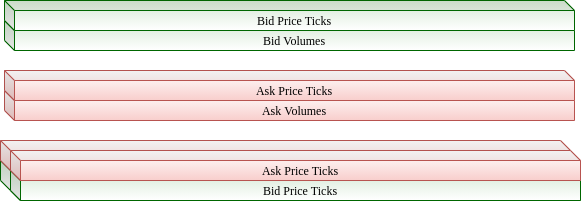
\includegraphics[width=1.0 \textwidth]{images/orderbook_structure}
	\centering
	\caption{نحوه‌ی جداسازی و ذخیره‌ی دفتر سفارشات	}
	\label{fig.orderbook_structure}
\end{figure}

\section{استخراج ویژگی و سری‌زمانی از دفتر سفارشات}
همانطور که در فصل قبل اشاره کردیم دفتر سفارشات را می‌توان به صورت دنباله‌ای از دوتایی‌های مرتب شامل قیمت و حجم متناظر در نظر گرفت. با جدا سازی دو بخش خرید و فروش و همچنین جداسازی دو بخش قیمت و حجم برای هر دفتر ثبت سفارش در طول زمان به یک آرایه‌ی سه بعدی که شامل تمامی اطلاعات دفتر سفارشات اولیه است دست پیدا می‌کنیم(شکل \ref{fig.orderbook_structure}). در این شکل آرایه‌ی سه بعدی مد نظر با ابعاد $2 * 2 * Depth$ نمایش داده شده است که $Depth$ یا عمق در آن به معنای تعداد سفارش‌های موجود در هر سمت دفتر سفارشات است. در این پروژه عمق دفتر سفارشات در هر دو سمت خرید و فروش را برابر در نظر می‌گیریم تا نمایش بهتری از داده‌ها داشته باشیم. هر دندانه‌ی\LTRfootnote{Tick} قیمتی به یک قیمت مشخص برای دارایی مورد مطالعه اشاره می‌کند. فواصل این دندانه‌ها توسط صرافی مربوطه تعیین می‌شود و گاها نسبت ثابتی با آخرین قیمت معامله‌شده دارد، اما عمدتا این فواصل به صورت ثابت و پیش‌فرض برابر مقدار کمی مانند ۱۰ سنت در نظر گرفته می‌شوند. علت این امر ایجاد انعطاف بیشتر برای خریداران و فروشندگان در سفارشات است. 

\subsection{دفتر سفارشات تجمعی}
در مرحله‌ی بعدی دفتر سفارشات تجمعی را تعریف می‌کنیم. هدف‌ اصلی از تعریف دفتر سفارشات تجمعی دستیابی به نمایش بهتری از عرضه و تقاضا نسبت به دفتر سفارشات عادی است\cite{blazejewski2004application}.\\
\begin{figure}[!t]
	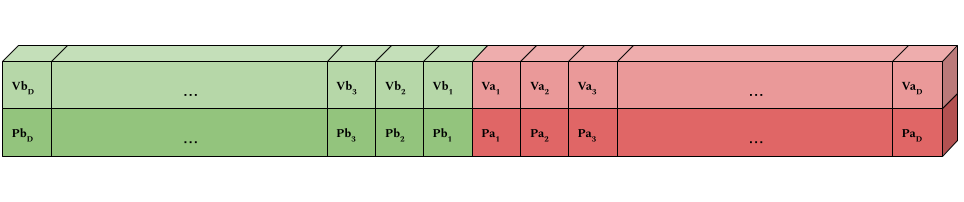
\includegraphics[width=1 \textwidth]{images/orderbook_t1}
	\centering
	\caption{اندیس گذاری دفتر سفارشات برای ایجاد دفتر سفارشات تجمعی	}
	\label{fig.orderbook_t1}
\end{figure}
حجم‌های تجمعی را بر اساس حجم‌های اولیه (شکل \ref{fig.orderbook_t1}) تعریف می‌کنیم:
\begin{equation}
	\begin{aligned}
			\bar{V}b_i = \sum_{j=1}^{i} Vb_j\\
			\bar{V}a_i = \sum_{j=1}^{i} Va_j
	\end{aligned}
\end{equation}
که $Vb_i$ و $\bar{V}b_i$ در آن به ترتیب بیانگر حجم خرید در دندانه‌ی $i$ام خرید و حجم تجمعی خرید در دندانه‌ی $i$ام هستند. به همین شکل، $Va_i$ و $\bar{V}a_i$ در آن به ترتیب بیانگر حجم فروش در دندانه‌ی $i$ام فروش و حجم تجمعی فروش در دندانه‌ی $i$ام هستند.\\
با تشکیل این دنباله‌های جدید، می‌توان تفسیر جدیدی برای دفتر سفارشات در نظر گرفت. در این نمایش جدید $\bar{V}$ها نشان دهنده‌ی حداکثر میزان حجم موجود برای خرید (یا فروش) در صورت تمایل به پرداخت (یا دریافت) قیمت متناظر با هر دندانه‌ هستند. بدین شکل هر دندانه‌ی سفارشی معنا‌ی کامل‌تری نسبت به حالت قبلی پیدا می‌کند چرا که محل قرارگیری سفارش‌های خریداران و فروشندگان در دفتر سفارشات در این نمایش جدید گنجانده شده‌است.\\
به طور مثال، قرار دادن یک سفارش خرید با حجم بسیار زیاد در نزدیکی بالاترین قیمت پیشنهادی خرید تمامی پیشنهادهای با قیمت کمتر را تحت تاثیر قرار می‌دهد و از احتمال اجرا شدن آن‌ها می‌کاهد. اینگونه سفارشات با حجم بالا که به عنوان دیوار قیمتی\LTRfootnote{Price Wall} شناخته می‌شوند از اهمیت بسیار زیادی برخوردار هستند چرا که وجود یا عدم وجودشان باعث تفسیر متفاوتی از سفارش‌های بعد از آنها می‌شوند.
\begin{figure}[!t]
	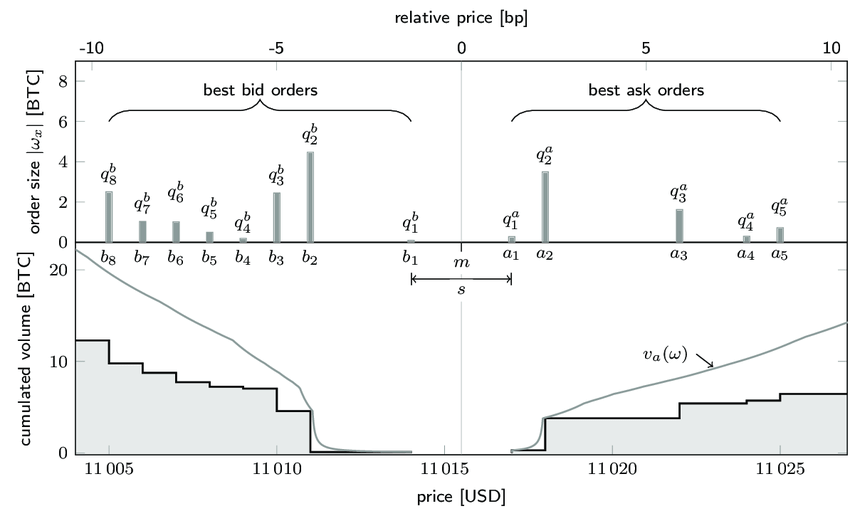
\includegraphics[width=1 \textwidth]{images/orderbook_t2}
	\centering
	\caption{نمونه‌ای از دفتر سفارشات معمولی و دفتر سفارشات تجمعی متناظر\cite{Schnaubelt2019}}
	\label{fig.orderbook_t2}
\end{figure}
\subsection{استخراج ویژگی‌های دیگر از دفتر سفارشات}
در این مرحله به استخراج برخی دیگر از ویژگی‌های دفتر سفارشات که در برخی از مطالعات انجام‌شده بر روی دفتر سفارشات از آن‌ها استفاده شده‌است می‌پردازیم.
\subsubsection{قیمت میانی}
قیمت میانی برای هر دفتر سفارشات به صورت میانگین بیشترین قیمت خرید و کمترین قیمت فروش در نظر گرفته می‌شود. این مقدار را به صورت زیر می‌توان تعریف کرد:
\begin{equation}
	MidPrice = \dfrac{(Pb_1 + Pa_1)}{2} 
\end{equation}
قیمت میانی می‌تواند تخمین خوبی از قیمتی که معامله‌ی بعدی در آن انجام می‌شود به دست دهد و از این جهت حائز اهمیت است.
\subsubsection{شکاف قیمت}
شکاف قیمت\LTRfootnote{Price Spread} اختلاف بین بالاترین قیمت خرید و پایین‌ترین قیمت فروش است. که به صورت زیر محاسبه می‌شود:
\begin{equation}
	PriceSpread = Pa_1 - Pb_1 
\end{equation}

\subsubsection{تغییر قیمت یا بازده}
مقدار تغییر قیمت که به آن بازده نیز گفته می‌شود، معمولا به صورت لگاریتمی در مطالعات استفاده می‌شود. این مقدار با استفاده از دو قیمت میانی متوالی قابل محاسبه است که به صورت مقابل نشان داده می‌شود:
\begin{equation}
	PriceChange_{t+1} = ln(\dfrac{MidPrice_{t+1}}{MidPrice_t}) = ln(MidPrice_{t+1})  - ln(MidPrice_t)
\end{equation}

\subsubsection{شکاف قیمتی وزن‌دار}
این مقدار بیانگر اختلاف موجود میان مجموع تقاضای خرید و فروش است. برای محاسبه‌ی این مقدار به طور معمول از ۱۰\% اول دفتر سفارشات استفاده می‌کنیم تا یک میانگین وزن‌دار از مجموع تقاضاهای خرید و فروش موجود در این بازه بسازیم. این مقدار را به صورت مقابل تعریف می‌کنیم:
\begin{equation}
	WheigtedSpread = \dfrac{1}{n}(\sum_{i=1}^{n}Pa_i * Va_i - \sum_{i=1}^{n}Pb_i * Vb_i)
\end{equation}
\vspace{-2em}
$$
	n = Depth / 10
$$
\newpage
\subsubsection{نوسان}
نوسان قیمت را نیز طبق فرمول \ref{eq:vol} برای پنجره‌های مختلف استخراج می‌کنیم و به مجموعه‌ داده ورودی برای هر نقطه اضافه می‌کنیم.
\subsection{استانداردسازی ویژگی‌ها}
در ادامه برای یادگیری بهتر لازم است تا ویژگی‌های استخراج‌شده را از نظر آماری استاندارد کنیم. یک ویژگی استاندارد داری میانگین صفر و واریانس یک است،‌ و برای استانداردسازی هر ویژگی باید ابتدا میانگین مقدار آن و انحراف معیار آن را در طول زمان را به دست بیاوریم و سپس طبق رابطه‌ی زیر ویژگی را استاندارد کنیم:
\begin{equation}
	X_{standard} = \dfrac{X - \bar{X}}{\delta}
\end{equation}
که $X$ بیانگر مقدار ویژگی در هر نقطه، $\bar{X}$ میانگین ویژگی $X$ در طول زمان و $\delta$ برابر انحراف معیار ویژگی $X$ است.
\section{یادگیری}
در این پروژه قصد داریم تا با استفاده از مدل‌های شبکه‌ی عصبی بازگشتی اقدام به یادگیری توزیع نوسان بر حسب ویژگی‌های استخراج شده کنیم. در این راستا، ابتدا شبکه‌های بازگشتی عمیق ساده را معرفی می‌کنیم و مشکلات آن‌ها را بررسی می‌کنیم. سپس به ساختار مدل جی‌آریو می‌پردازیم و راه حل این مدل برای مشکلات گفته شده را بررسی می‌کنیم. در انتها نحوه‌ی یادگیری بر اساس نمونه‌ها توسط این مدل را تشریح می‌کنیم.
\subsection{شبکه‌های عصبی بازگشتی}
شبکه‌های عصبی بازگشتی برای یادگیری داده‌هایی که طبیعت دنباله‌ای دارند طراحی شده‌اند\cite{weigend1990predicting}. این شبکه‌ها به دلیل ساختار دنباله‌ای در زمینه‌های مختلفی مانند پردازش زبان طبیعی و همچنین پیش‌بینی سری‌های زمانی به صورت گسترده استفاده شده‌اند.
\begin{figure}[!t]
	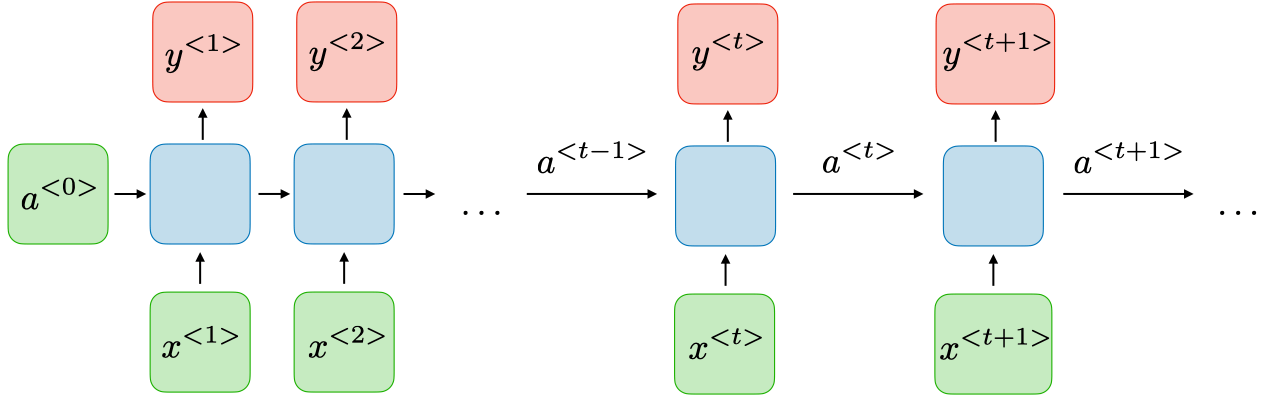
\includegraphics[width=1 \textwidth]{images/rnn_1}
	\centering
	\caption{شمای کلی شبکه‌های عصبی بازگشتی}
	\label{fig.rn1}
\end{figure}
این شبکه‌ها یک دنباله‌ی ورودی از داده‌ها را می‌گیرند و دنباله‌ای دیگر به عنوان خروجی تولید می‌کنند.\\
برای هر نقطه‌ی زمانی $t$، تابع فعال‌سازی $\alpha^{<t>}$ و تابع خروجی $y^{<t>}$ به صورت زیر محاسبه می‌شوند:
\begin{equation}
	\label{eq:rnn1}
	\alpha^{<t>} = g_1(W_{aa}\alpha^{<t-1>} + W_{ax}x^{<t>} + b_a)
\end{equation}
\vspace{-4em}
\begin{equation}
	\label{eq:rnn2}
	y^{<t>} = g_2(W_{ya}a^{<t>} + b_y)
\end{equation}
که ماتریس‌های $b_a$، $b_y$، $W_{ya}$، $W_{aa}$ و $W_{ax}$ در آن ضرایبی هستند که توسط هر سلول به اشتراک گذاشته می‌شود. از طرفی $g_1$ و $g_2$ نیز توابع فعال‌سازی\LTRfootnote{Activation Function} هستند که در ادامه با آن‌ها خواهیم پرداخت.
\begin{figure}[!t]
	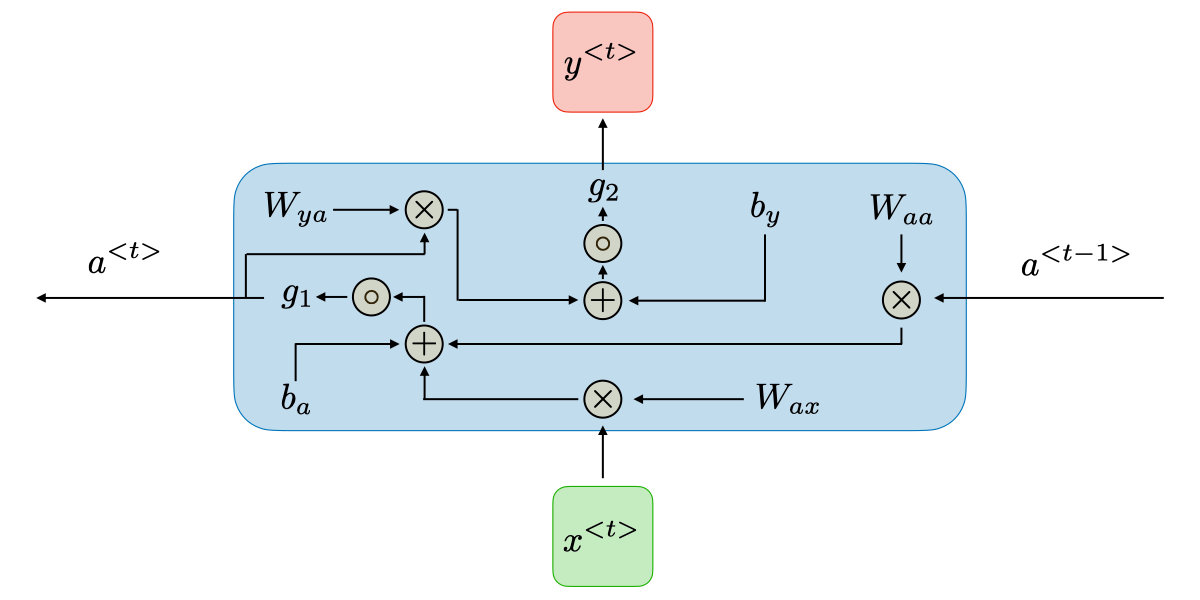
\includegraphics[width=0.8 \textwidth]{images/rnn_cell}
	\centering
	\caption{نمایی از روابط \ref{eq:rnn1} و \ref{eq:rnn2} که نحوه‌ی محاسبات انجام شده درون هر سلول شبکه‌ی عصبی بازگشتی را نشان می‌دهند.}
	\label{fig.rncell}
\end{figure}
\newpage
استفاده از شبکه‌های عصبی بازگشتی مزایا و معایب متفاوتی دارد که در ادامه به آن‌ها اشاره می‌کنیم.
\subsubsection{معایب شبکه‌های بازگشتی}
همانطور که پیش‌تر گفته شد. شبکه‌های عصبی بازگشتی از مشکل از بین رفتن گرادیان رنج می‌برند\cite{hochreiter1998vanishing}. این مسئله از تضعیف مقدار گرادیان در انتقال بین سلول‌ها ناشی می‌شود. هنگامی که فاصله‌ی نقطه‌ای که خطا در آن محاسبه شده با یک سلول زیاد می‌شود، گرادیان خطا نسبت به متغیرهای آن سلول مقدار بسیار کمی می‌گیرند که مانع از انجام یادگیری توسط مدل می‌شود. این مسئله باعث می‌شود تا ارتباطات بلندمدت در دنباله‌ی ورودی توسط مدل یاد گرفته نشود. در ادامه خواهیم دید که شبکه‌ی جی‌آریو چگونه با استفاده از حافظه‌ی داخلی این مشکل را برطرف می‌کند.\\
از طرف دیگر، به دلیل انتقال یک طرفه‌ی اطلاعات در این شبکه‌ها، امکان انتقال خطا از سلول‌های جلویی به عقبی وجود ندارد و به همین دلیل ورودی‌های بعدی در وضعیت فعلی متغیرهای سلول تاثیری نخواهند داشت. هرچند این مسئله در پیش‌بینی سری‌های زمانی خیلی مطرح نیست چرا که اغلب بر اساس دنباله‌ای از داده‌های ثبت شده در یک بازه‌ی زمانی به پیش‌بینی نقطه‌های بعدی می‌پردازیم. اما این مشکل در پردازش زبان طبیعی بسیار حائز اهمیت است که موجب پیدایش شبکه‌ها بر پایه توجه\LTRfootnote{Attention} شده‌است.
\subsubsection{مزایای شبکه‌های بازگشتی}
این شبکه‌ها به خاطر به اشتراک‌گذاری وزن‌ها در طول زمان، نسبت به افزایش طول ورودی حساسیتی ندارند و با افزایش طول ورودی تعداد پارامتر‌های آن‌ها افزایش نمیابد. این ویژگی این شبکه‌ها را برای استفاده در مسائل پیش‌بینی سری‌های زمانی که گاهی دارای ورودی بسیار بزرگ هستند مناسب می‌کند.\\
از طرفی، با به اشتراک‌گذاری وزن‌ها بین سلول‌ها، به نوعی دانش موجود برای نقاط مختلف زمانی به اشتراک گذاشته می‌شود، که باعث به وجود‌ آمدن مدل‌های کاراتری می‌شود. اطلاعات و خروجی توابع فعال‌سازی سلول‌های قبلی نیز در هر سلول به کار گرفته می‌شوند که ویژگی بسیار مناسبی در پیش‌بینی سری‌های زمانیست.\\
\newpage
\subsection{جی‌آریو}
جی‌آریو گونه‌ای از شبکه‌های عصبی بازگشتیست که برای حل مسئله‌ی گردایان از بین رونده و مدل‌سازی روابط طولانی مدت در داده‌های ورودی به وجود آمده است. این شبکه‌ها با استفاده از ساختاری مشابه به حافظه اقدام به حفظ اختیاری اطلاعات سلول‌های گذشته و انتقال آن‌ها به سلول‌های بعدی می‌کنند.\\
\begin{figure}[!t]
	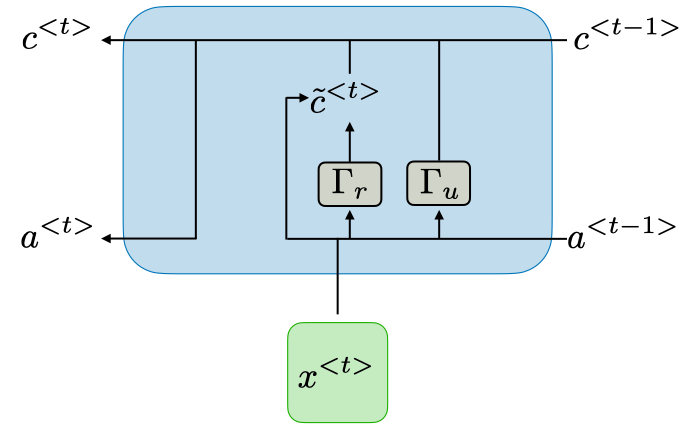
\includegraphics[width=0.8 \textwidth]{images/gru_1}
	\centering
	\caption{ساختار داخل هر سلول از شبکه‌ی عصبی جی‌آریو.}
	\label{fig.gru_1}
\end{figure}
برای متوجه شدن بهتر نحوه‌ی کارکرد این مدل از شبکه‌های عصبی روابط ریاضی آن‌ها را تشریح می‌کنیم:
\begin{equation}
	\tilde{c}^{<t>} = tanh(W_c[\Gamma_r * \alpha^{t-1} , x^{<t>}] + b_c)
\end{equation}
\vspace{-4em}
\begin{equation}
	\tilde{c}^{<t>} = tanh(W_c[\Gamma_r * \alpha^{t-1} , x^{<t>}] + b_c)
\end{equation}
\vspace{-4em}
\begin{equation}
	a^{<t>} = c^{<t>}
\end{equation}
که $\Gamma$ در آن مشخص کننده‌ی دروازه‌هاست که هرکدام هدف مشخصی دارند. رابطه ریاضی برای هر دروازه به صورت زیر است:
\begin{equation}
	\Gamma = \sigma(Wx^{<t>} +Ua^{<t-1>} + b)
\end{equation}
که $b$، $U$ و $W$ ضرایب متناظر با هر دروازه هستند و $\sigma$ تابع سیگموید است. که به صورت زیر تعریف می‌شود:
\begin{equation}
	\sigma(x) = \dfrac{1}{1 + e^{-x}}
\end{equation}
در هر سلول جی‌آریو $\Gamma_r$ مشخص کننده میزان ارتباط اطلاعات ورودی جدید در زمان $t$ است و به آن‌ دروازه‌ی ربط گفته می‌شود. این دروازه مشخص می‌کند که تا چه میزان اطلاعات ورودی جدید وارد حافظه‌ی بلندمدت یا همان متغیر $\tilde{c}$ بشود. از طرف دیگر، $\Gamma_u$ مشخص می‌کند که اطلاعاتی که از قبل درون حافظه وجود داشته اند تا چه میزان باید فراموش شوند و چه میزان از آن‌ها باید حفظ شود و ازین جهت به آن دروازه‌ی به‌روزرسانی گفته می‌شود.
\subsection{تابع خطا}
معیار‌های مختلفی برای گزارش خطا در پیش‌بینی سری‌های زمانی وجود دارد. تعریف تابع خطا در مطالعات بر روی سری زمانی اهمیت بسیار زیادی دارد، چرا که توابع خطا‌ی مختلف نتیجه‌های بسیار متفاوتی در مدل‌ نهایی به وجود می‌آورند. به طور مثال، توابع خطایی که با داده‌های پرت\LTRfootnote{Outlier} مانند باقی داده‌ها رفتار می‌کنند نتیجه‌ی قابل قبولی در مدل نهایی ارائه نمی‌دهند، چرا که این داده‌ها در سری‌های زمانی عموما غیر قابل پیش‌بینی هستند و به همین خاطر می‌توانند خطای قابل توجهی را به مدل‌ها تحمیل کنند. از طرف دیگر، هدف از به کار گیری مدل نوسان داشتن تخمین خوبی از نوسان در طول زمان به صورت عمومیست و نه فقط بازه‌های خاصی که پیش‌بینی ‌نوسان در آن‌ها بسیار سخت است،‌ به همین خاطر سعی در طراحی و استفاده از تابع خطا، جهت‌دهی یادگیری به سمتی است که در تعداد زیادی از نقاط تخمین خوبی از دنباله‌ی هدف توسط مدل حاصل شود. از همین جهت انواع مختلفی از توابع خطا در این حوزه به کار گرفته ‌شده‌اند که در ادامه به معرفی تعدادی از آن‌ها می‌پردازیم.
\newpage
\subsubsection{میانگین مربعات خطا}
این معیار خطا که به نوعی از نرم دوم خطا استفاده می‌کند،‌ با جمع زدن و میانگین‌گیری از مربعات خطا، معیاری از دقت عملکرد سیستم گزارش می‌دهد که رابطه‌ی آن به صورت زیر است:
\begin{align}
	\vcenter{\hbox{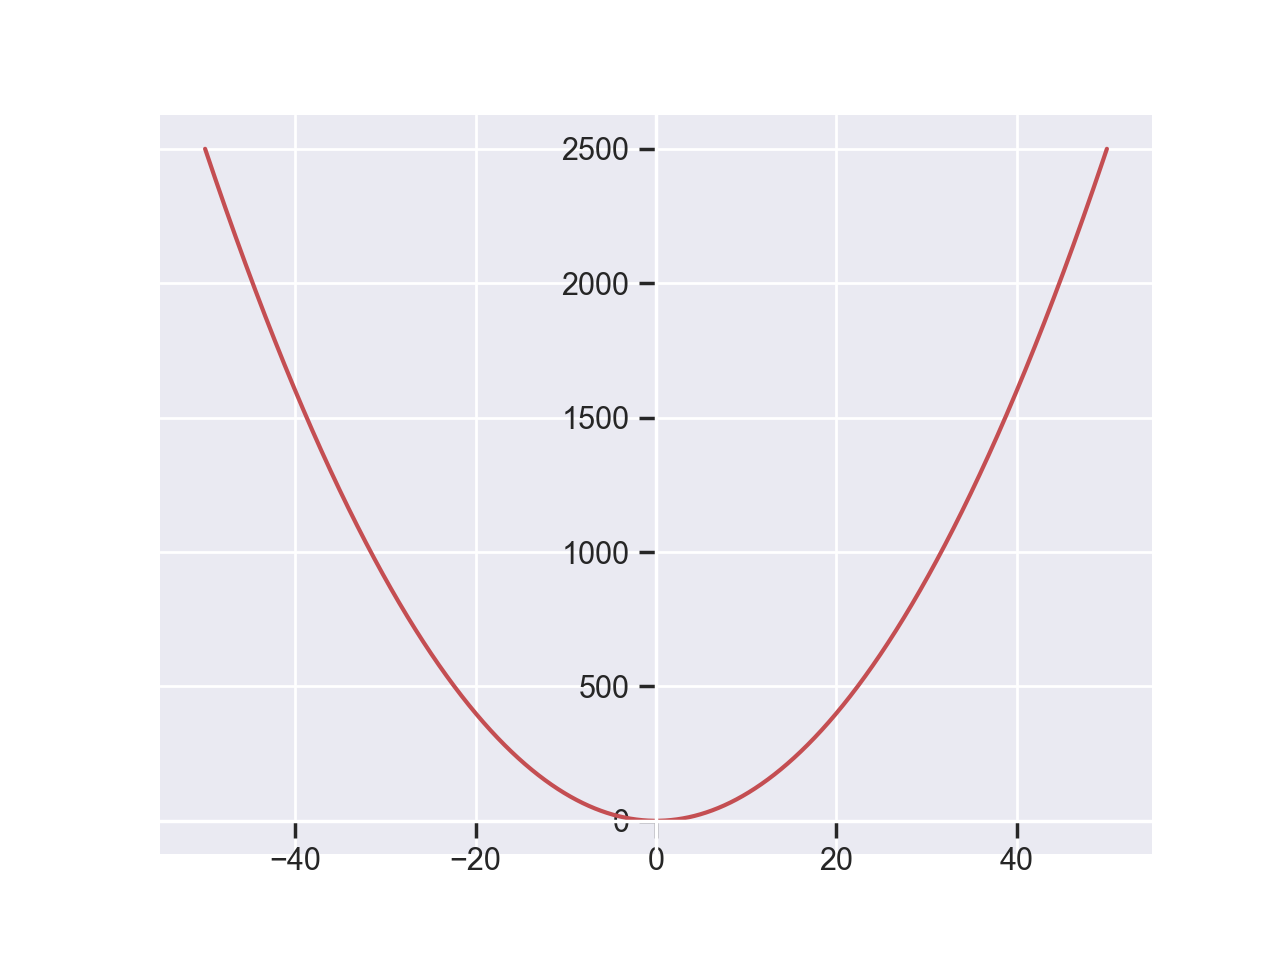
\includegraphics[width=6cm,height=6cm]{images/MSE}}}
	&\qquad\qquad
	\begin{aligned}
		MSE = \dfrac{1}{n} \sum_{i=1}^{n}(Y_i - \hat{Y}_i)^2
	\end{aligned}\\
	\vcenter{\hbox{\begin{minipage}{6cm}
				\captionof{figure}{نمودار تابع میانگین مربعات خطا بر اساس میزان خطا یا $\epsilon$}
	\end{minipage}}}
	& \notag
\end{align}
این تابع خطا نسبت به داده‌های پرت بسیار حساس بوده و ازین جهت جای بهبود دارد.

\subsubsection{میانگین قدرمطلق خطا}
این معیار خطا که به نوعی از نرم اول خطا استفاده می‌کند،‌ با جمع زدن از قدر مطلق خطا، معیاری از دقت عملکرد سیستم گزارش می‌دهد که رابطه‌ی آن به صورت زیر است:
\begin{align}
	\vcenter{\hbox{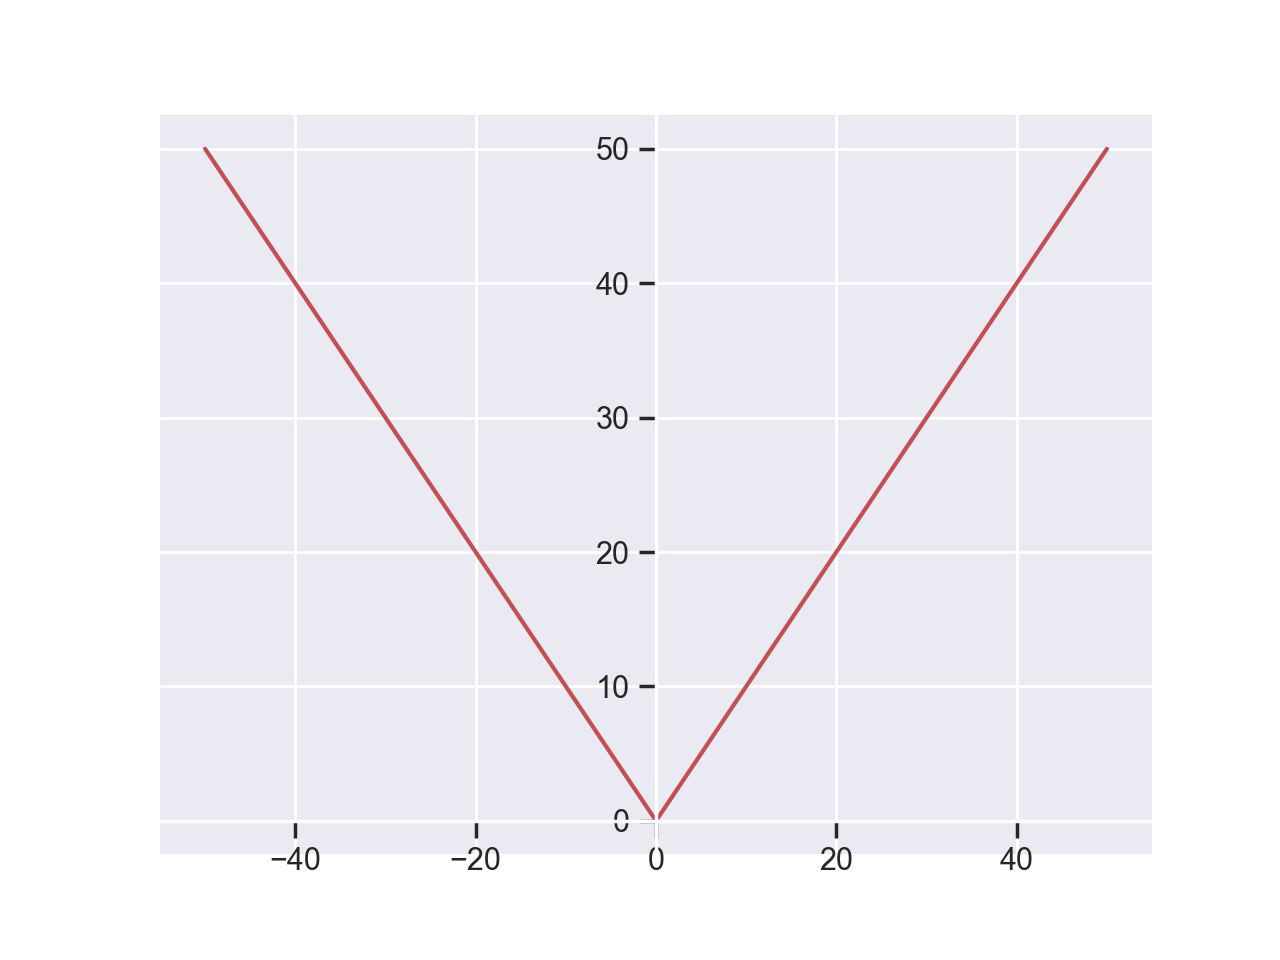
\includegraphics[width=6cm,height=6cm]{images/MAE}}}
	&\qquad\qquad
	\begin{aligned}
		MAE = \dfrac{1}{n} \sum_{i=1}^{n}|Y_i - \hat{Y}_i|
	\end{aligned}\\
	\vcenter{\hbox{\begin{minipage}{6cm}
				\captionof{figure}{نمودار میانگین قدرمطلق خطا بر اساس میزان خطا یا $\epsilon$}
	\end{minipage}}}
	& \notag
\end{align}
میانگین قدر مطلق خطا نسبت به تمامی نقاط موجود در مجموعه داده‌ رفتار یکسانی دارد. علت این امر آن است که شیب نمودار خطا به ازای تمامی مقادیر $\epsilon$ ثابت است و مانند میانگین مجموع مربعات خطا برای داده‌ها پرت افزایش نمیابد. ازین جهت می‌توان گفت که این تابع خطا نسبت به داده‌ها پرت حساسیت کمتری دارد.

\subsubsection{میانگین نسبی قدرمطلق خطا}
میانگین نسبی قدرمطلق خطا\LTRfootnote{Mean Absolute Percentage Error} مانند میانگین قدرمطلق خطا از نرم اول خطا برای محاسبه‌ی هزینه‌ی نهایی استفاده می‌کند، اما در مقابل این خطا را به مقدار ورودی اصلی تقسیم می‌کند که باعث می‌شود نوعی عادی سازی\LTRfootnote{Normalization} صورت بگیرد. رابطه‌ی این تابع خطا به صورت زیر است:
\begin{equation}
	MAPE = \dfrac{1}{n} \sum_{i=1}^{n}|\dfrac{Y_i - \hat{Y}_i}{\hat{Y}_i}|
\end{equation}
میانگین نسبی قدرمطلق خطا تابع خطای مناسبی برای سری‌های زمانی است. سری‌های زمانی اغلب با افزایش و کاهش‌های شدید در طول زمان مواجه هستند. در مقابل پیش‌بینی‌های انجام‌شده بر روی هر سری زمانی با خطاهایی همراه هست که با مقدار سری زمانی در آن نقطه نسبت مستقیمی دارند. به بیان دیگر با افزایش مقدار یک سری زمانی در طول زمان(به عنوان مثال افزایش نوسان بازار) پیش‌بینی آن با همان میزان خطای مطلق قبلی بسیار دشوارتر می‌شود و در نتیجه میزان خطای مدل نیز افزایش پیدا می‌کند. این مسئله باعث می‌شود تا مقادیر بزرگتر سری زمانی خطای بیشتری نسبی به مقادیر کوچک‌تر به مدل تحمیل کنند.\\
برای حل این مشکل تابع میانگین نسبی قدرمطلق خطا پیشنهاد شده است که با تقسیم مقدار مطلق خطا به مقدار سری زمانی در آن نقطه معیار بهتری از عملکرد سیستم نسبت به توابع دیگر به دست می‌دهد. از نگاهی دیگر این تابع خطا نسبت به افزایش و کاهش سری‌زمانی حساس نیست که باعث می‌شود خطای یکنواختی در طول سری زمانی ارائه کند. 
\newpage
\section{جمع‌بندی}
در این فصل با نحوه‌ی استخراج ویژگی‌ها مختلف از دفتر سفارشات آشنا شدیم و سپس به معرفی شبکه‌های عصبی بازگشتی و ساختار آن‌ها پرداختیم. در انتها نیز توابع خطای مورد استفاده در مطالعه‌ی سری‌های زمانی را معرفی کردیم. در فصل بعدی روش و جزییات پیاده سازی را تشریح می‌کنیم.

